\chapter{Einführung und Ziele}

\section{Aufgabenstellung}

Es soll ein verteiltes Steuerungssystem gemäß den Prinzipien verteilter Systeme nach Tanenbaum \& van Steen entworfen und implementiert werden. Über ein ITS-Board (bspw. STM32F4) soll ein autonomer Roboter innerhalb eines kontrollierten Areals (z.B. BT7 R7.65 – als realer Testbereich) sicher und effizient gesteuert werden. Die verteilte Architektur soll dabei explizit gewährleisten, dass durch Fehlverhalten der Software oder Architektur keine Gefahr für anwesende entstehen kann.


\section{Qualitätsziele}
% Aus VS Skript Kapitel 2.4 Seite 23
% TODO zu jeden Punkt eine Definition oder entfernen
% TODO messbar definieren

Das verteilte Steuerungssystem soll eine Reihe von nicht-funktionalen Anforderungen erfüllen, um einen sicheren, wartbaren und erweiterbaren Betrieb im Einsatzumfeld zu gewährleisten. 

\subsection{Ziele für Software Engineering}
\begin{table}[h!]
    \centering
    \begin{tabular}{p{4cm}|p{5cm}|p{5cm}|}
        \hline
        \textbf{Ziel} & \textbf{Beschreibung} & \textbf{Metrik} \\
        \hline
        Funktionalität &  
        %Der Roboter muss Steuerbefehle korrekt umsetzen, auf Umgebungsdaten reagieren und vordefinierte Aufgaben zuverlässig erfüllen.
        & Alle Abnahmetests werden erfolgreich bestanden
        \\
        \hline
        Zuverlässigkeit & 
        %Teilausfälle dürfen den Gesamtsystembetrieb nicht gefährden. Fehlererkennung und -toleranz müssen integriert sein.
        & Das System ist über dem gesamten Abnahmezeitraum stabil (ca. 1,5 h)
        \\
        \hline
        Skalierbarkeit & 
        %Zusätzliche Roboter oder Komponenten sollen ohne Änderungen an der bestehenden Architektur integrierbar sein. 
        & Es können beliebig viele Roboter hinzugefügt und entfernt werden (0 - N)
        \\
        \hline
        Leistung & 
        %Reaktionszeiten auf Steuerbefehle und Ereignisse müssen innerhalb definierter Zeitgrenzen liegen. 
        & Reaktionszeit max. 500 ms
        \\
        \hline
        Sicherheit (Safety) & 
        %Das System darf unter keinen Umständen eine Gefährdung für Personen/Gegenstände darstellen. Bei Fehlern muss sofort ein sicherer Zustand erreicht werden (z.B. Notstopp). 
        & Reaktionszeit max. 500 ms
        \\
        \hline
        Wartbarkeit & 
        %Der Code muss modular, gut dokumentiert und testbar sein. Fehlerdiagnose und Protokollierung sollen integriert sein. 
        & 
        \\
        \hline
        Portabilität & %Die Software soll ohne großen Aufwand auf vergleichbaren Embedded-Systemen lauffähig sein. 
        & nicht relevant
        \\
        \hline
        Benutzerfreundlichkeit & %Konfiguration und Überwachung müssen intuitiv bedienbar und gut visualisiert sein. 
        & Keine Einweisung erforderlich
        \\
        \hline
        Anpassbarkeit & 
        %Neue Funktionen, Sensoren oder Regeln sollen ohne tiefgreifende Änderungen am System integrierbar sein. 
        & 
        \\
        \hline
        Kompatibilität & 
        %Das System soll mit bestehenden Standards und Protokollen kommunizieren können. 
        & 
        \\
        \hline
    \end{tabular}
    \caption{Qualitätsziele der Software Engineering}
    \label{tab:seziele}
\end{table}

\clearpage
\subsection{Ziele der Verteilte Systeme}
    \begin{table}[h!]
        \centering
        \begin{tabular}{p{4cm}|p{5cm}|p{5cm}|}
            \hline
            \textbf{Ziel} & \textbf{Beschreibung} & \textbf{Metrik} \\
            \hline
            Ressourcenteilung  & ...& \\
            Offenheit & ...& \\
            Skalierbarkeit & ...& siehe Tabelle \ref{tab:skalierbarkeit} \\
            Verteilung Transparenz & ...& siehe Tabelle \ref{tab:transparenzen} \\
            \hline
        \end{tabular}
        \caption{Qualitätsziele der Verteilten Systeme}
        \label{tab:vsziele}
    \end{table}
    
\subsubsection{Skalierbarkeit}
    \begin{table}[h!]
            \centering
            \begin{tabular}{p{4cm}|p{5cm}|p{5cm}|}
                \hline
                \textbf{Ziel} & \textbf{Metrik} & \textbf{Metrik} \\
                \hline
                Vertikale Skalierung   & ... &\\
                \hline
                Horizontale Skalierung & ...& \\
                \hline
                Räumliche Skalierbarkeit &  & 1 \\
                \hline
                Funktionale Skalierbarkeit & ... & \\
                \hline
                Administrative-Skalierbarkeit & &1 \\
                \hline
            \end{tabular}
            \caption{Skalierbarkeit von verteilten Systemen}
            \label{tab:skalierbarkeit}
        \end{table}
    
\newpage
\subsubsection{Verteilungs-Transparenzen}
    \begin{table}[h!]
            \centering
            \begin{tabular}{p{4cm}|p{5cm}|p{5cm}|}
                \hline
                \textbf{Ziel} & \textbf{Beschreibung} & \textbf{Metrik} \\
                \hline
                Zugriffstransparenz   & ...&\\
                \hline
                Lokalitäts-Transparenz  & ...&\\
                \hline
                Migrationstransparenz & ...&\\
                \hline
                Replikationstransparenz &...&\\
                \hline
                Fehlertransparenz &... &\\
                \hline
                Ortstransparenz & .. &\\
                \hline
                Skalierbarkeits-Transparenz & ... & \\
                %Concurrency
                %Relocation
                \hline
            \end{tabular}
            \caption{Verteilungs-Transparenzen}
            \label{tab:transparenzen}
        \end{table}
        



\clearpage
\section{Stakeholder}
Die folgenden Gruppen sind direkt oder indirekt vom System betroffen:

\begin{itemize}
    \item \textbf{Endnutzer:} Personen, die mit dem Roboter interagieren (z.B. Lehrpersonal, Kinder im Testbereich)
    \item \textbf{Entwicklerteam:} Zuständig für Entwurf, Umsetzung, Tests und Wartung des Systems
    \item \textbf{Betreiber:} Verantwortlich für die Überwachung und den sicheren Betrieb des Systems im realen Umfeld
    \item \textbf{Professor:} Person, die für die Bewertung des Systems verantwortlich ist und vorgabe der Rahmenbedingungen.

\end{itemize}


\subsection*{Use Case Diagramm} % TODO make this the label/caption

\begin{figure}[h]
	\centering
	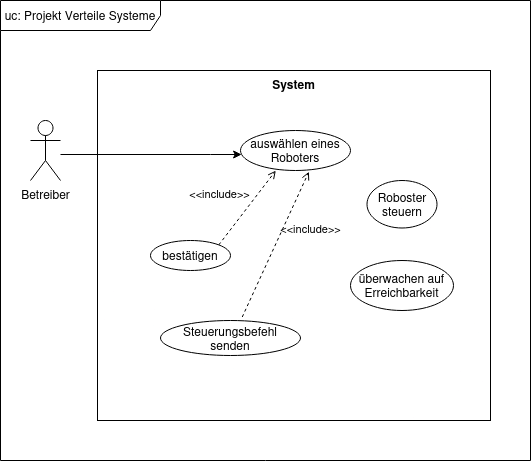
\includegraphics[scale=.5]{diagrams/use_case.png}
	\caption{Funktionales Use Case Diagramm der Aufgabenstellung}
	\label{fig:meine-grafik}
\end{figure}
